\documentclass{article}
\usepackage{graphicx} % Required for inserting images
\usepackage{amsmath}  % For mathematical equations
\usepackage{lipsum}   % For generating dummy text
\usepackage{titling}  % For customizing title
\usepackage{xcolor}   % For custom colors
\usepackage{enumitem} % For customizing itemized lists
\usepackage{geometry} % For adjusting page margins
\usepackage{fancyhdr} % For custom headers and footers
\usepackage{titlesec} % For custom section formatting
\usepackage{setspace} % For custom line spacing

% Define custom colors
\definecolor{darkblue}{RGB}{0,0,128}

% Set page margins
\geometry{margin=1in}

% Custom title formatting
\renewcommand{\maketitle}{
  \begin{center}
    
\includegraphics[width=7cm]{iithlogo.png} % Replace 'iit_hyderabad_logo.png' with the actual logo filename and path
    \vspace{1cm}
    
    {\LARGE\bfseries\textcolor{darkblue}{Design Elements }} \\[1ex]
    {\LARGE\bfseries\textcolor{darkblue}{Analog and Integrated Circuits}}
    
    \vspace{1cm}
    
    \large\textcolor{darkblue}{Abhishek Amit Raje} \\
    \thedate
  \end{center}
}

% Custom section formatting
\titleformat{\section}[block]{\LARGE\bfseries\color{darkblue}}{\thesection}{1em}{}
\titlespacing*{\section}{0pt}{\baselineskip}{0.5\baselineskip}

% Customized list
\newlist{myitemize}{itemize}{1}
\setlist[myitemize,1]{label=\textcolor{darkblue}{\textbullet},left=1em}

% Define header and footer
\pagestyle{fancy}
\fancyhf{} % Clear default header and footer
\rhead{\thepage} % Page number on the right header
\lfoot{\textcolor{darkblue}{Analog and Integrated Circuits}} % Left footer
\cfoot{} % Center footer
\rfoot{\textcolor{darkblue}{Abhishek Amit Raje}} % Right footer
\renewcommand{\headrulewidth}{0pt} % Remove header rule line

% Set line spacing
\onehalfspacing

\begin{document}

\begin{titlingpage}
  \maketitle
\end{titlingpage}

\section{Problem Statement}
We are required to build an LED blinker for the Neuromodulation lab that blinks every time a pulse is generated by the SoC. We must also make sure that the blinking is captured by the camera placed 15 feet away.

\section{Approach Taken}
The approach taken to light the LEDs would be to use the Mosfet as a voltage-dependent current source to power the LEDs that are connected in parallel. The Gate of the Mosfet will be connected to the (GPIO) pin of an SoC, and the source will be connected to the Ground.

\begin{equation}
V_{gs} = 3.3\text{V}
\end{equation}

Then we will connect the drain to the resistor, and the other end of the resistor is connected to the cathode of the LED while the anode is connected to the SoC, which implies:

\begin{equation}
V_{ds} = 5\text{V}
\end{equation}

\section{Simulation of the System}
\begin{figure}[h]
  \centering
  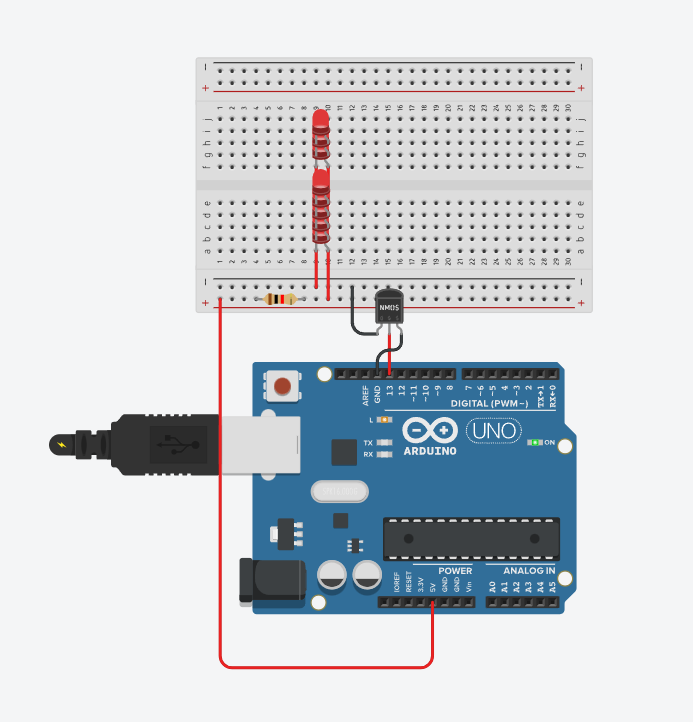
\includegraphics[width=0.5\textwidth]{Mosfet_sol.png} % Change 'Mosfet_sol.png' to your image file name
  \caption{Arduino Simulation of the Circuit}
  \label{fig:arduino_simulation}
\end{figure}

\section{Mosfet Characteristics}
\begin{figure}[h]
  \centering
  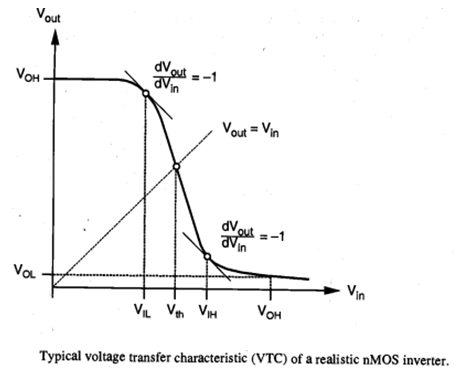
\includegraphics[width=0.7\textwidth]{MosfetInputOutput.png} % Change 'MosfetInputOutput.png' to your image file name
  \caption{Voltage Transfer Characteristics of a Mosfet}
  \label{fig:mosfet_characteristics}
\end{figure}

As we can observe from the graph, the minimum value of \(V_{in}\) is \(V_{th}\), and the maximum value of \(V_{in}\) is \(V_{th} + \frac{-1 + \sqrt{1 + 2V_s kR}}{kR}\) for the Mosfet to operate in the saturation zone. The value of \(V_s\) and \(R\) must be taken such that \(V_{gs}\) lies within the range of \(V_o\).

The overall benefit of using this system over directly connecting the LEDs is direct control over \(i_{ds}\) by changing the gate voltage.

the forward voltage of the LED is between 1.2 to 3.6 V, and the forward current is between 10 to 30 mA.
\begin{align}
80\,\text{mA} & < I_d = \frac{k}{2} (V_{gs} - V_t)^2 < 240\,\text{mA}
\end{align}
\section{Limitations in Design}
There would be a voltage drop across the drain of the Mosfet:
\[
V_{o} = V_{s} - i_{d}R
\]
This can lead to a decrease in the brightness of LEDs depending on the voltage drop.

The Mosfet may heat up due to excessive current passing through it. Power is also dissipated by the current-limiting resistor connected across the LED.

\section{Powering the SoC}
There are several options for powering the Arduino-based SoC:

\begin{itemize}
  \item \textbf{USB Power:} Most Arduino boards can be powered via a USB connection from a computer or a USB wall adapter. The board has an onboard voltage regulator that steps down the USB voltage to the required voltage.
  
  \item \textbf{Battery Power:} You can power an Arduino using batteries, such as AA or AAA batteries, through the onboard voltage regulator or directly, depending on the Arduino model.
\end{itemize}
\section{Modeling the Problem}
\begin{itemize}
  \item Ideal Voltage Source (SoC GPIO):
    \begin{itemize}
      \item The SoC's GPIO pin can be represented as an ideal voltage source.
      \item It provides a control voltage to the gate of the MOSFET.
    \end{itemize}
    
  \item MOSFET Model:
    \begin{itemize}
      \item The Mosfet in the saturation zone can be modeled as a voltage-dependent current source.
    \end{itemize}
    
  \item Resistor:
    \begin{itemize}
      \item The resistor connected in series with the LED can be modeled as an ideal resistor.
    \end{itemize}
    
  \item LEDs (Light Emitting Diodes):
    \begin{itemize}
      \item LEDs can be approximated as ideal diodes.
      \item They have no voltage drop across them in this assumption.
      \item We have assume the LED's to have linear V-I characteristics even though they have non linear V-I characteristics 
    \end{itemize}
\end{itemize}
\begin{figure}[h]
  \centering
  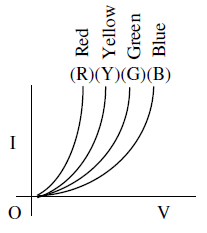
\includegraphics[width=0.3\textwidth]{LEDV-I chARECTERISTICS.png} % Change 'MosfetInputOutput.png' to your image file name
  \caption{I-V Characteristics of a  LED}
  \label{fig:mosfet_characteristics}
\end{figure}
The Link of the TinkerCad Simulation \href{https://shorturl.at/yM147}

\end{document}
